\chapter{Introduction} \label{chapter_1}

\chapterprecishere{``Quote"\par\raggedleft--- \textup{Who said it}, Where}

\utsinitial{T}his is a chapter. Maybe introductory. 
You can use your pre-defined acronyms like this. \Gls{ACR}. or \gls{aCP} if you want to retain the capitalization of the first letter. \Gls{Abbr} will still print the regular abbreviation. Only those abbreviations used will be shown in the list. You can also add some sections and cite stuff \cite{citation1}. 

\section{The PhD process at BUW}
You can add figures like Figure \ref{fig_BUW_process}. Or tables such as Table \ref{tab:my_label}

\begin{figure}
    \centering
    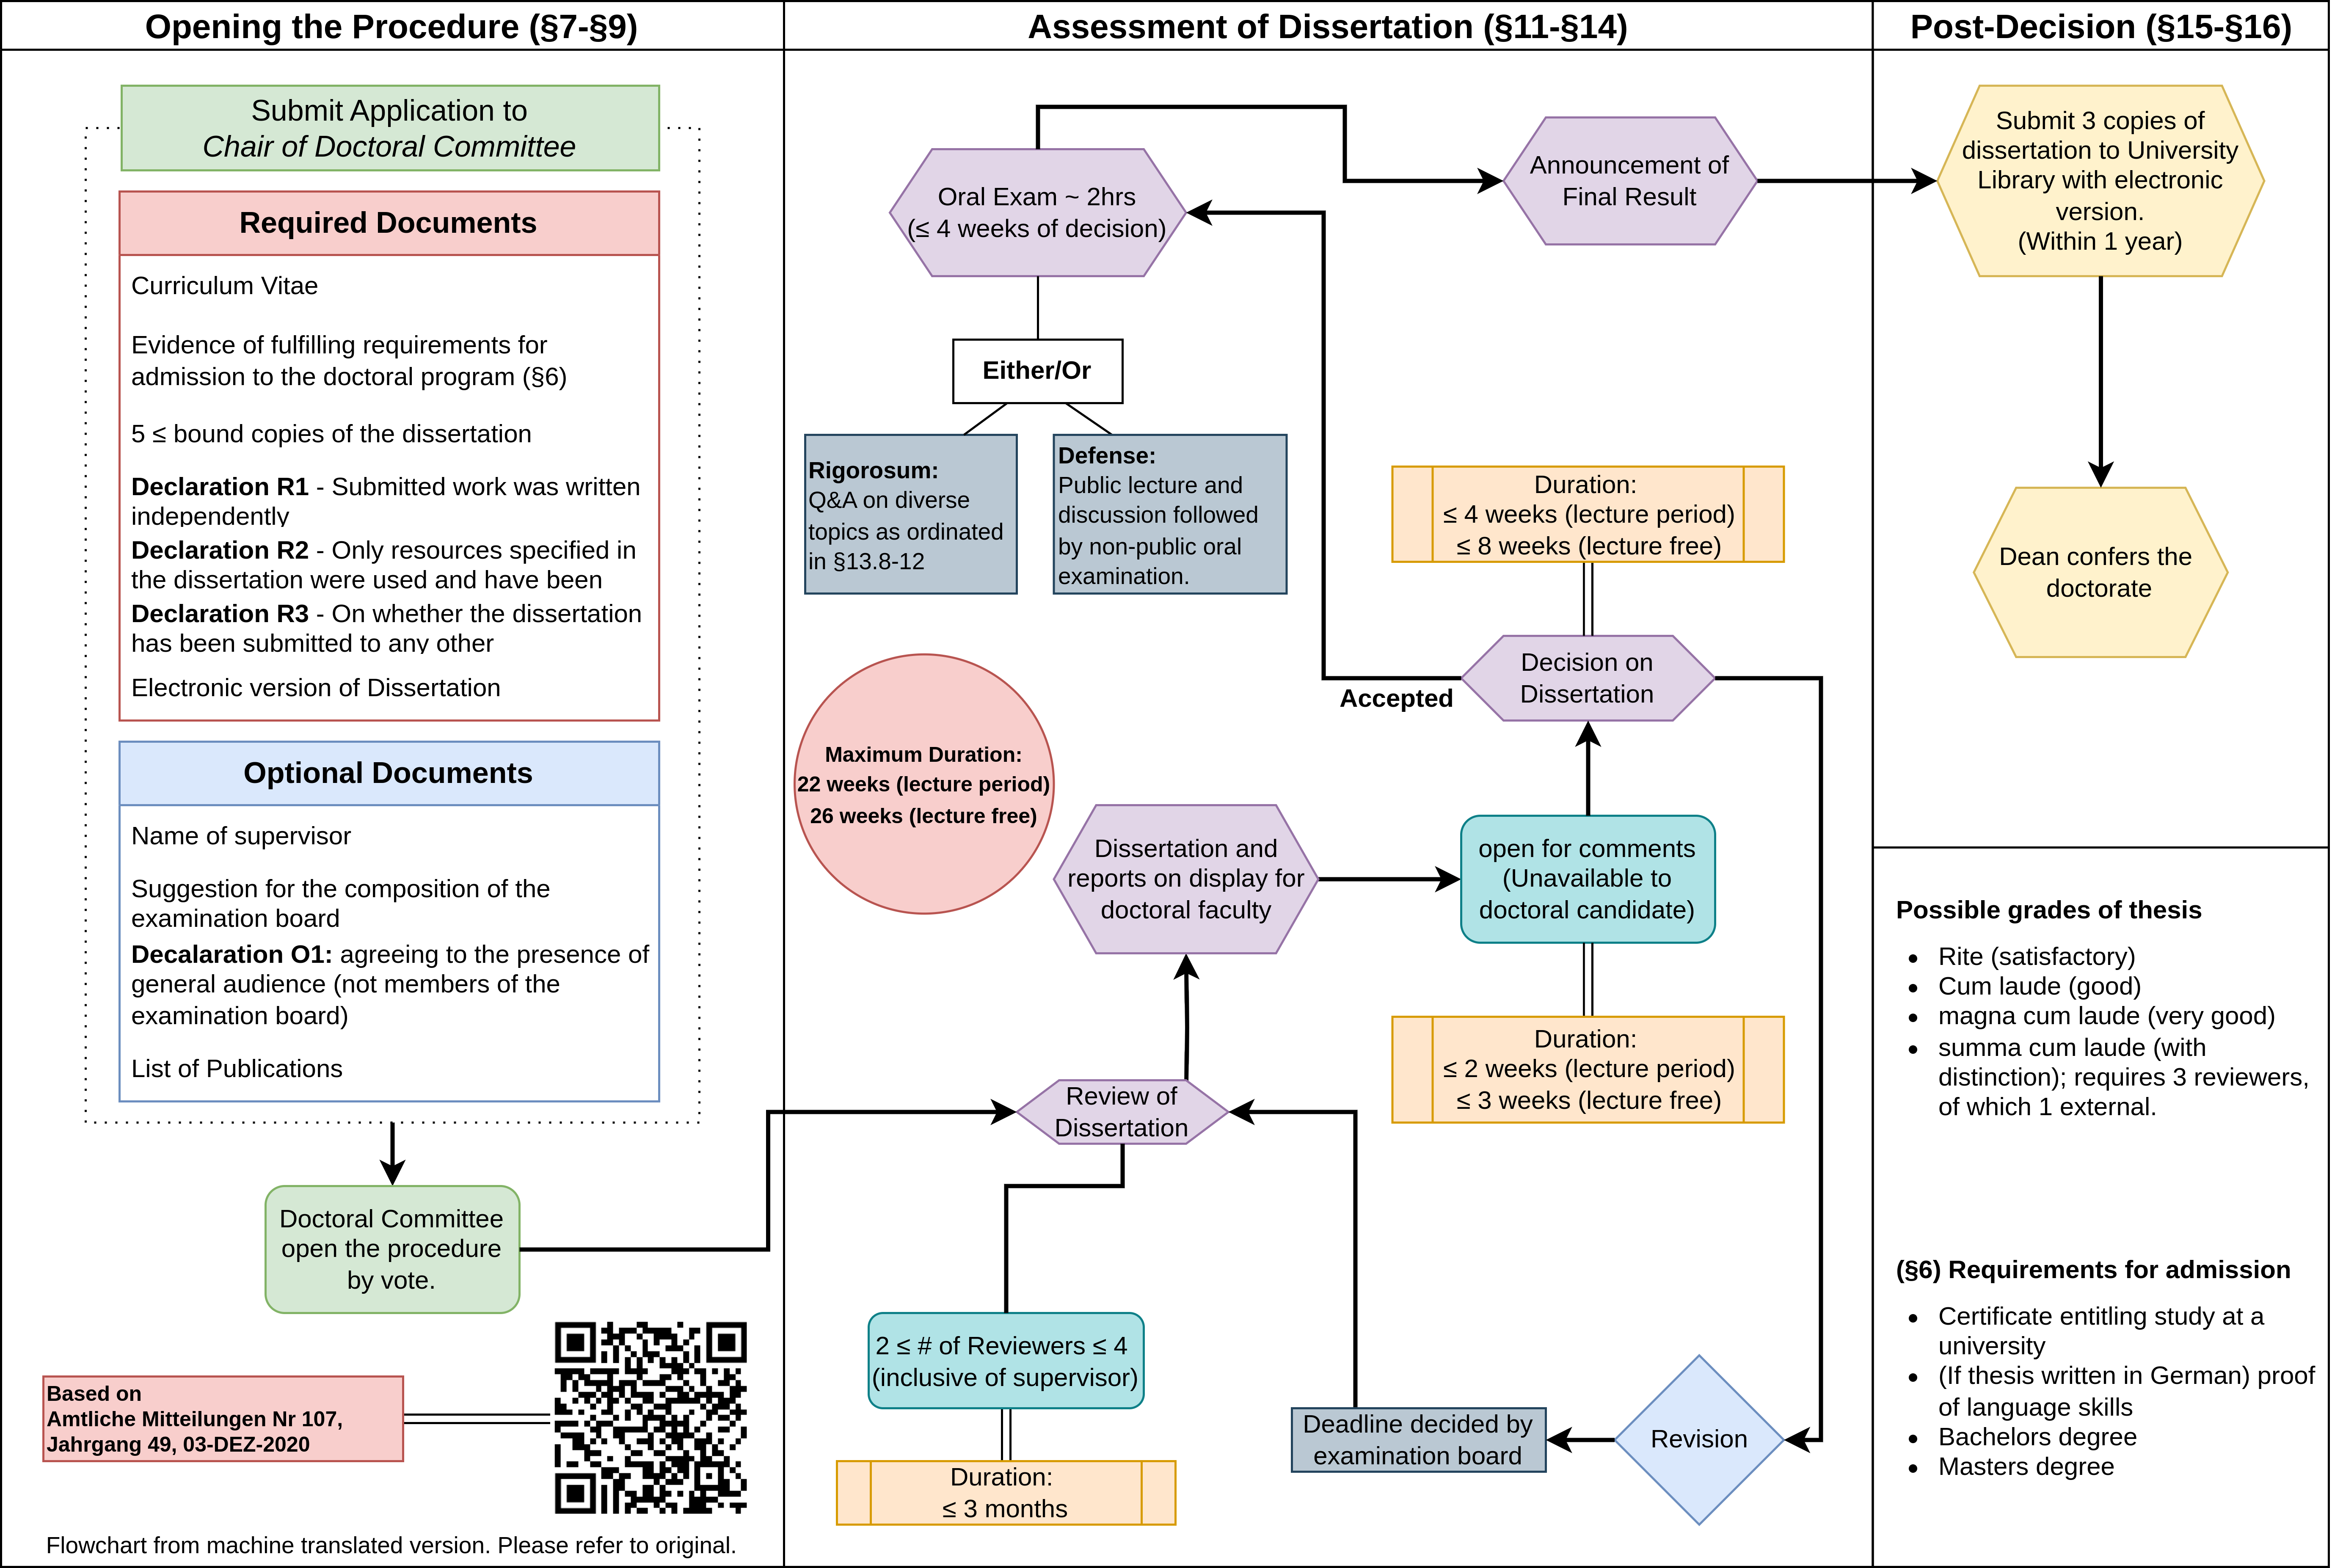
\includegraphics[width=\linewidth]{assets/PhDProcess.png}
    \caption[Short caption for TOC]{Some long caption: \lipsum[2-2]}
    \label{fig_BUW_process}
\end{figure}


\begin{table}[htb!]
    \centering
    \begin{tabular}{c|c}
        bb & cc \\
         aa & aa
    \end{tabular}
    \caption[TOC caption]{Long caption for table.}
    \label{tab:my_label}
\end{table}